\documentclass[aspectratio=43,english]{beamer} %If you want to create Polish presentation, replace 'english' with 'polish' and uncomment 3-th line, i.e., '\usepackage{polski}'
\usepackage[utf8]{inputenc}
\usepackage{polski} %Uncomment for Polish language
\usepackage{babel}
\usepackage{listings} %We want to put listings

\mode<beamer>{ 	%in 'beamer' mode
	\hypersetup{pdfpagemode=FullScreen}		%Enable Full screen mode
	\usetheme{JuanLesPins} 		%Show part title in right footer
	%\usetheme[dark]{AGH}                 		%Use dark background
	%\usetheme[dark,parttitle=leftfooter]{AGH}  	%Use dark background and show part title in left footer
}
\mode<handout>{	%in 'handout' mode
	\hypersetup{pdfpagemode=None}		
	\usepackage{pgfpages}
  	\pgfpagesuselayout{4 on 1}[a4paper,border shrink=5mm,landscape]	%show 4 slides on 1 page
  	\usetheme{boxes}
  	\addheadbox{structure}{\quad\insertpart\hfill\insertsection\hfill\insertsubsection\qquad} 	%content of header
 	\addfootbox{structure}{\quad\insertauthor\hfill\insertframenumber\hfill\insertsubtitle\qquad} 	%content of footer
}

\AtBeginPart{ %At begin part: display its name
	\frame{\partpage}
} 


%%%%%%%%%%% Configuration of the listings package %%%%%%%%%%%%%%%%%%%%%%%%%%
% Source: https://en.wikibooks.org/wiki/LaTeX/Source_Code_Listings#Using_the_listings_package
%%%%%%%%%%%%%%%%%%%%%%%%%%%%%%%%%%%%%%%%%%%%%%%%%%%%%%%%%%%%%%%%%%%%%%%%%%%%
\lstset{ %
  backgroundcolor=\color{white},   % choose the background color
  basicstyle=\footnotesize,        % the size of the fonts that are used for the code
  breakatwhitespace=false,         % sets if automatic breaks should only happen at whitespace
  breaklines=true,                 % sets automatic line breaking
  captionpos=b,                    % sets the caption-position to bottom
  commentstyle=\color{green},      % comment style
  deletekeywords={...},            % if you want to delete keywords from the given language
  escapeinside={\%*}{*)},          % if you want to add LaTeX within your code
  extendedchars=true,              % lets you use non-ASCII characters; for 8-bits encodings only, does not work with UTF-8
  frame=single,	                   % adds a frame around the code
  keepspaces=true,                 % keeps spaces in text, useful for keeping indentation of code (possibly needs columns=flexible)
  keywordstyle=\color{blue},       % keyword style
  morekeywords={*,...},            % if you want to add more keywords to the set
  numbers=left,                    % where to put the line-numbers; possible values are (none, left, right)
  numbersep=5pt,                   % how far the line-numbers are from the code
  numberstyle=\tiny\color{gray},   % the style that is used for the line-numbers
  rulecolor=\color{black},         % if not set, the frame-color may be changed on line-breaks within not-black text (e.g. comments (green here))
  showspaces=false,                % show spaces everywhere adding particular underscores; it overrides 'showstringspaces'
  showstringspaces=false,          % underline spaces within strings only
  showtabs=false,                  % show tabs within strings adding particular underscores
  stepnumber=2,                    % the step between two line-numbers. If it's 1, each line will be numbered
  stringstyle=\color{cyan},        % string literal style
  tabsize=2,	                   % sets default tabsize to 2 spaces
  title=\lstname,                  % show the filename of files included with \lstinputlisting; also try caption instead of title
                                   % needed if you want to use UTF-8 Polish chars
  literate={?}{{\k{a}}}1
           {?}{{\k{A}}}1
           {?}{{\k{e}}}1
           {?}{{\k{E}}}1
           {�}{{\'o}}1
           {�}{{\'O}}1
           {?}{{\'s}}1
           {?}{{\'S}}1
           {?}{{\l{}}}1
           {?}{{\L{}}}1
           {?}{{\.z}}1
           {?}{{\.Z}}1
           {?}{{\'z}}1
           {?}{{\'Z}}1
           {?}{{\'c}}1
           {?}{{\'C}}1
           {?}{{\'n}}1
           {?}{{\'N}}1
}
%%%%%%%%%%%%%%%%%


\title{Metody Obliczeniowe w Nauce i Technice}
\author{Marian Bubak, PhD}
\date{}
\institute[AGH]{
	Institute of Computer Science\\ul. Kawiory 21\\30-055 Krakow\\
	Poland\\
	\url{http://www.icsr.agh.edu.pl/~mownit/}
}



% Powtarzam oznaczenie równania "(*)" w różnych punktach jako nowe oznaczenie. Czy tak jest dobrze, czy zamienić na unikalne w obrębie prezentacji?

\subtitle{12. Iteracyjne rozwiązywanie Ax=B}
\setcontributors{Anna Marciniec\\Radosław Kazior\\Łukasz Janeczko}


\begin{document}
  \maketitle
	\begin{frame}{Plan wykładu}
		\tableofcontents
	\end{frame}

  \section{12.1 Wady metod bezpośrednich}

\begin{frame}{Wady metod bezpośrednich}
  \begin{block}{\textbf{Złożoność obliczeniowa} ${\sim}N^3$}
    \begin{itemize}
      \item{ $M=\frac{1}{3}n^3+n^2-\frac{1}{3}n$ ($\cdot$,$/$)}
      \item{ $D=\frac{1}{3}n^3+\frac{1}{2}n^2-\frac{5}{6}n$ ($+$)}
    \end{itemize}
    Np. $10^4$ punktów siatki przestrzennej (mesh points)
    \begin{itemize}
      \item{100 x 100   (2 -- D)}
      \item{20 x 20 x 20   (3 -- D)}
      \item{metoda eliminacji Gaussa to $\sim 10^{12}$ operacji}
      \item{1 operacja trwa $\sim 10^{-8}$ s.}
      \item{$10^4$ czyli $\sim$ 3 godziny}
    \end{itemize}
  \end{block}
\end{frame}

\begin{frame}{}
  \begin{block}{\textbf{Zwykle}}
    \begin{itemize}
      \item{czas symulacji $\sim$ 1h,}
      \item{liczba kroków czasowych $\sim$ 1000,}
      \item{cały krok - to rozwiązywanie układu równań,}
      \item{1 operacja $\sim 10^{-8}$ s,}
      \item{liczba punktów siatki $\sim 10^4$ ($\equiv$ liczba równań)}
    \end{itemize}
  \end{block}
\end{frame}

\begin{frame}{}
  \begin{block}{\textbf{Potrzebne są metody o znacznie mniejszej złożoności}}
    Metody takie powinny być oparte na własnościach równań różniczkowych cząstkowych (zwykle - źródła równań liniowych):
    \begin{itemize}
      \item{liniowość,}
      \item{wymiar,}
      \item{możliwość separacji zmiennych,}
      \item{zakres zmian współczynników,}
      \item{kształt geometryczny obszaru,}
      \item{warunki brzegowe - postać.}
    \end{itemize}
  \end{block}
\end{frame}

\begin{frame}{}
  \textbf{Metody bezpośrednie zaburzają strukturę macierzy rzadkich}
  \newline 2 - D $\rightarrow$ operator pięciopunktowy
  \begin{figure}
    \centering
    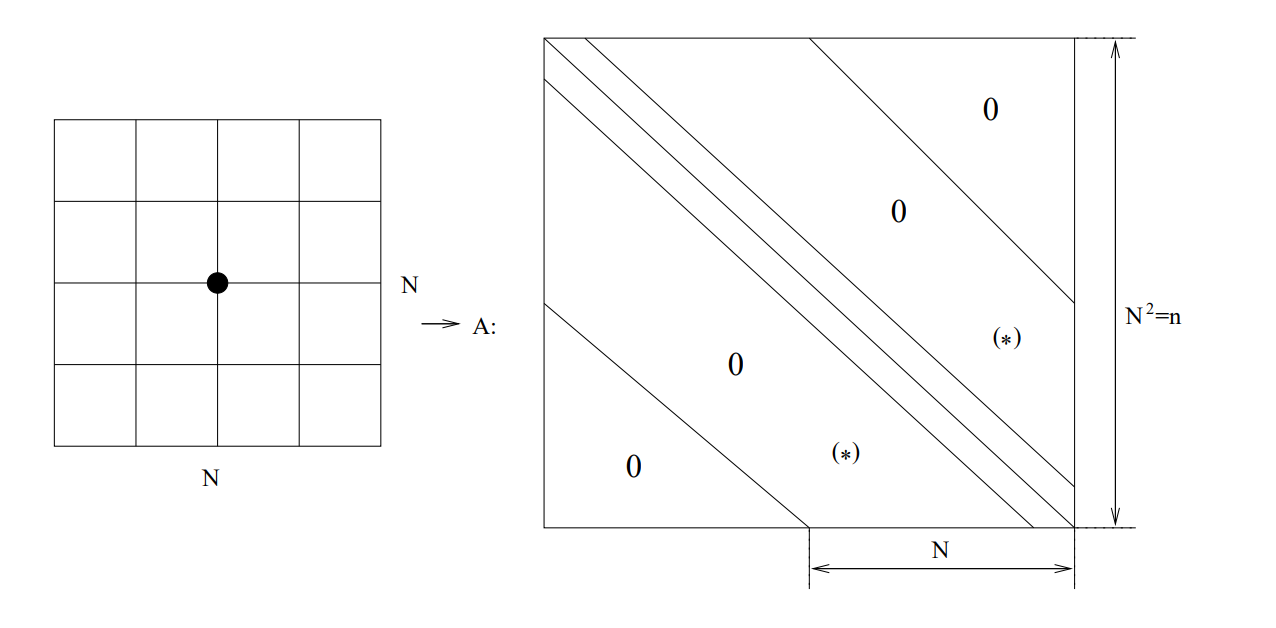
\includegraphics[height=0.75\textheight, width=1.1\textwidth]{img/12/iteracja1}
  \end{figure}
\end{frame}

\begin{frame}{}
  \begin{block}{\textbf{Metody bezpośrednie zaburzają strukturę macierzy rzadkich}}
    \begin{itemize}
      \item{$\sim 5 \cdot N^2$ współczynników $\neq$ 0}
      \item{ale: po zastosowaniu metody eliminacji Gaussa znikają zera z wstęg
      \newline (*) $\rightarrow$ trzeba wtedy pamiętać $2 \cdot N^3$ współczynników}
      \item{Macierz wstęgowa: $m_{ij}=0$ dla $|i-j|>k$}
      \item W metodach polegających na mnożeniu $A \cdot x^{(t)}$ w kroku t zamiast $n^2 \rightarrow k \cdot n$ mnożeń $\Rightarrow$ wtedy łatwo o:
      \begin{center}
      $s \cdot k \cdot n<n^3$
      \end{center}
      \item gdzie s - liczba kroków, a $n^3$ - złożoność metod bezpośrednich.
    \end{itemize}
  \end{block}
\end{frame}


  \section{12.2 Podział metod iteracyjnych}

\begin{frame}{Podział metod iteracyjnych}
  \begin{block}{\textbf{Metody stacjonarne} (\emph{stationary})}
    \begin{itemize}
      \item stałe współczynniki macierzy iteracyjnej,
      \item starsze,
      \item proste w zrozumieniu i implementacji,
      \item na przykład metody Jacobiego, G--S (SR), SOR, SSOR.
    \end{itemize}
  \end{block}
\end{frame}

\begin{frame}{}
  \begin{block}{\textbf{Metody niestacjonarne} (\emph{nonstationary})}
    \begin{itemize}
      \item współczynniki macierzy iteracyjnej zmieniają się w kolejnych krokach iteracji,
      \item oparte na idei
      \begin{itemize}
        \item ciągu wektorów ortogonalnych (CG, MINRES ...),
        \item wielomianów ortogonalnych (metoda Czybyszewa),
      \end{itemize}
      \item stosunkowo nowe,
      \item trudniejsze w zrozumieniu i implementacji,
      \item szybciej zbieżne.
    \end{itemize}
  \end{block}
\end{frame}

\begin{frame}{}
  \begin{block}{}
    \emph{iterate} -- przybliżenie rozwiązania w kolejnej iteracji,
    \newline \emph{residual} -- $r=Ay-b$,
    \newline \emph{preconditioner, preconditioning matrix:} macierz transformująca układ równań do postaci o lepszych własnościach spektralnych
  \end{block}
\end{frame}


  \section{12.3 Istota metod iteracyjnych dla Ax=b}

\begin{frame}{Istota metod iteracynych dla Ax=b}
    \begin{center}
      $A*x=b\quad(1)$
    \end{center}
    \begin{itemize}
      \item gdzie A jest macierzą n x n;
      \item x -- wektor n niewiadomych;
      \item b -- wektor danych (źródeł)
    \end{itemize}
\end{frame}

\begin{frame}
  \begin{block}{\textbf{Rozkład:}}
      $$A=B+R$$
    \begin{itemize}
      \item B -- macierz dla, której łatwo $B^{-1}$
      \item R -- pozostałość
    \end{itemize}
    $\Rightarrow$
    $$B*x=-R*x+b$$<++>
  $$\boxed{B*x=-(A-B)*x+b}\quad(2)$$
  \end{block}
\end{frame}

\begin{frame}{}
    \textbf{Metody iteracyjne dla Ax = b (mesh relaxation methods) polegają na:}
    \begin{itemize}
      \item odgadnięciu wektora początkowego $x^{(o)}$
      \item generowaniu ciągu iteracyjnego $x^{(t)}$ wg. postulowanego wzoru:
    \end{itemize}
    $$B*x^{(t+1)}=-(A-B)*x^{(t)}+b \hskip \textwidth minus \textwidth (12.1)$$
    $$x^{(t+1)}=\underbrace{-B^{-1}*(A-B)}_{I-B^{-1}*A=M \quad M - iteration matrix} *x^{(t)}+\underbrace{B^{-1}*b}_{W}\quad(3) \hskip \textwidth minus \textwidth (12.2)$$
\end{frame}

\begin{frame}{}
    \textbf{Różne B $\rightarrow$ rodzina metod iteracyjnych:}
    $$\boxed{x^{(t+1)}=M*x^{(t)}+B^{-1}*b}\quad(4)$$
    Warunek \emph{zgodności} formuły iteracyjnej z szukanym rozwiązaniem
    $$\lim_{t\to\infty} x^{(x+1)}= \lim_{t\to\infty}  (M*x^{(t)}+B^{-1}*b) \quad (5)$$
\end{frame}



  \section{12.4 Zbieżność procesu iteracyjnego rozwiązywania Ax=b}

\begin{frame}{Zbieżność procesu iteracyjnego rozwiązywania Ax=b}
  \textbf{Twierdzenie: Zbieżność procesu iteracyjnego}
  \begin{block}{Teza:}
    \center Ciąg ($\star$) z dowolnym wektorem startowym $x^{(0)}$ jest zbieżny do jedynego granicznego $x^{(\inf)}$ wtedy i tylko wtedy, gdy \emph{promień spektralny (sectral radius)} macierzy iteracji jest mniejszy od 1
    \center $\rho(M)<1$
  \end{block}
\end{frame}

\begin{frame}{}
  \begin{block}{Dowód}
    $\varepsilon^{(t)}=x^{(t)}-x$; wektor błędu w iteracji t
    \[\underbrace{x=M \cdot x+W\ oraz\ x^{(t+1)}}_{\varepsilon^{(t+1)}=M \cdot \varepsilon^{(t)} \Rightarrow \varepsilon^{(t)}=M^t \cdot \varepsilon^{(0)}}=M \cdot x^{(t)}+W\]
    (7) $\varepsilon^{(0)}$ - \emph{initial error vector} gdy M zmienia się w procesie iteracji - to:
    \[{\varepsilon}^{(t)}=M^t \cdot {\varepsilon}^{(0)} \quad (8)\]
    \emph{Dla określenia zbieżności - potrzebny jest skalar $||\varepsilon^{(t)}||$}.
    Chcemy, by dla pewnego $t$:
    \[||\varepsilon^{(t+1)}||<||\varepsilon^{(t)}||\]
  \end{block}
\end{frame}

\begin{frame}{}
  \begin{block}{Dowód}
    M -- macierz iteracji ma n różnych wartości i wektorów własnych
    \\\hfill$Ms_i=\rho _is_i$\hfill (12.3)
    \newline
    \\Rozkładamy (rzuty na inne osie):
    \\\hfill\[\varepsilon^{(t)}=M^t \sum_{i = 1}^{n} \alpha _i s_i , \alpha _i \text{ - amplituda kierunku } s_i\]\hfill (12.4)
    \[\varepsilon^{(t)}=M^t \sum_{i = 1}^{n} \alpha _i s_i = \sum_{i = 1}^{n} \alpha _i M^{t-1}(\underbrace{Ms_i}_{\rho _i s_i}) = ... = \sum_{i = 1}^{n} \alpha _i \rho _i^t s_i \]
    \[\boxed{\varepsilon^{(t)}=\sum_{i = 1}^{n} \alpha _i \rho _i^t s_i} \qquad (12.5)\]
  \end{block}
\end{frame}

\begin{frame}{}
  \begin{block}{Dowód}
    \[\lim_{t\to\infty} \varepsilon^{(t)} = \alpha _m \rho _m^t s_m\]
    gdzie: $\rho _m = max_i |\rho _i|= \rho$ promień spektralny macierzy iteracji
    \center \textbf{$\rho < 1$ - warunek zbieżności}
    $$ \frac{||\varepsilon^{(t)}||}{||\varepsilon^{(0)}||} \leq ||M^{(t)}|| \text{ - zadana dokładność } \rho\Rightarrow ||M^{(t\star)}|| = 10^{-p}$$   %TO CHECK - sprawdź oznaczenia!
    \\$\lambda$ -- \emph{asymptotic convergence factor}
    \[\lambda^{t\star}=10^{-p} \rightarrow t\star = -p \cdot  \frac{ln 10}{ln \lambda} \text{ - liczba iteracji}\]    %TO CHECK - there was a star near t
  \end{block}
\end{frame}


  \section{12.5 Sens procedury iteracyjnej dla Ax=b}

\begin{frame}{Sens procedury iteracyjnej dla Ax=b}
  W każdym kroku następuje poprawianie rozwiązania.\\
  Przypadek, gdy źródłem Ax=b jest r. Poissona :
  \begin{itemize}
    \item \fbox{$\bigtriangledown^2u(x,y)=-\rho(x,y)$}
    \item $\rho(x,y)$ -- f. rozkładu źródeł
    \item $\infty$ szybkość propagacji informacji
  \end{itemize}
\end{frame}

\begin{frame}{}
  Ale r. Poissona to graniczny (stacjonarny) przypadek \emph{równania dyfuzji} :
  $$\boxed{\frac{\partial u}{\partial t} = \bigtriangledown^2u=\rho}$$
  którego jawne sformułowanie różnicowe ma postać:
  $$
  \left.
  \begin{array}{lr}
    \text{siatka t}:\\
    t\rightarrow p,\\
    t+\Delta t\rightarrow p+1
  \end{array}\right|
  \underbrace{u^{(p+1)}=u^{(p)}+\Delta t\Delta^{||}y^{(p)}}_{Mu^{(p)}}+\underbrace{\rho\Delta t}_{W=B^{-1}b}
  $$
  

  Procedura iteracyjna- jawne rozwiązanie zagadnienia opisującego zbieżność w wyimaginowanym czsie iteracji (pseudoczas)
\end{frame}



  \section{12.6 Metoda Jacobiego}

\begin{frame}{Metoda Jacobiego}
  $$ A=D+(L+U);\{M=I-D^{-1}AW=D^{-1}b $$
  gdzie: L --poddiagonalna; P -- naddiagonalna;\\
  D=B -- diagonalna, z diagonalnych elementów macierzy A. Korzystając z zależności
  $$\boxed{Dx^{(t+1)}= -(L+U)x^{(t)}+b}$$
  otrzymujemy wzór roboczy:
  $$x_i^{(t+1)}=\frac{1}{a_{ij}}[b_i-\sum_{j/1\,j\neq i}^{n} a_{ij}x_j^{(t)}]/ ;/ a_{ij} \neq 0,\wedge i,$$
\end{frame}

\begin{frame}
  \begin{block}{Procedura przestawiania wierszy}
    \begin{itemize}
      \item[1.] spośród kolumn z $a_{ii} = 0$ wybieramy tą, która ma najwięcej zer,
      \item[2.] w tej kolumnie wybieramy element o max $|a_{ii}|$ i przestawiamy wiersze tak, aby znalazł się on na diagonali,
      \item[3.] Powtarzamy 1. i 2.
    \end{itemize}
  \end{block}
\end{frame}

\begin{frame}{}
  \begin{block}{Modelowe zadanie}
    równanie Poissona
    \\2-D
    \\w.b. $\Rightarrow\phi\equiv 0$
    \\siatka przestrzenna \emph{N x N}
  \end{block}

  \begin{block}{Dla modelowego zadanie -- met. Jacobiego:}
    $$\rho - cos\frac{\pi}{N}\approx 1 0 \frac{\pi^2}{N^2}, \lambda _J = \rho$$
  \end{block}
\end{frame}

\begin{frame}{}
  \begin{block}{Charakterystyka metody Jacobiego}
    \begin{itemize}
      \item prosta,
      \item znaczenie dydatkyczne,
      \item wolnozbieżna,
      \item nie wykorzystuje całej, dostępnej w danym kroku informacji,
      \item pamiętane $x^{(t)}$ i $x^{(t+1)}$,
      \item zbieżna dla A silnie diagonalnie dominujących,
      $$\text{wierszowo : }|a_{ii} > \sum_{j/1\neq i}^{n} |a_{ij},$$
      $$\text{kolumnowo : }|a_{ii} > \sum_{j/1\neq i}^{n} |a_{ji},$$
    \end{itemize}
  \end{block}
\end{frame}


  \section{12.7 Metoda Gaussa-Seidla (G-S i S-R -successive relaxation)}

\begin{frame}{}
  $$A=\underbrace{(L+D)}_{B}+U$$
  $$M=I-B^{-1}A=I-B^{-1}(B+U)=-B^{-1}U$$
  $$x^{(t+1)}=-B^{-1}Ux^{(t)}+B^{-1}b$$
  $$(D+L)x^{(t+1)}=-Ux^t+b$$
  $$\boxed{Dx^{(t+1)}=-Lx^{(t+1)}-Ux^{(t)}+b}$$
  i wzór roboczy
  $$x^{(t+1)}_i=\frac{1}{a_{ii}}[b_i-\underbrace{\sum^{i-1}_{j/1} a_{ij}x^{(t+1)}_j}_{(\star)}-\underbrace{\sum^{n}_{j/i+1} a_{ij}x^{(t)}_{j}}_{(\star\star)}]$$
  gdzie: ($\star$) - otrzymujemy z rozwiązania poprzednich równań w bieżącej (t + 1) iteracji i w tym tkwi przewaga nad m. Jacobiego i źródło wzrostu efektywności, ($\star\star)$ - z poprzedniej iteracji (t).
\end{frame}

\begin{frame}{}
  \begin{block}{Charakterystyka metody G-S}
    \begin{itemize}
      \item elementy diagonali powinny być $\neq$ 0 $\rightarrow$ przestawianie
      \item wystarczy pamiętać aktualne przybliżenie $x^{(t+1)}$
      \item zbieżna dla A:
      \begin{itemize}
        \item[*] silnie diagonalnie dominujących wierszowo, kolumnowo,
        \item[*] symetrycznych,
        \item[*] dodatnio określonych $(xAx>O\wedge x\neq 0)$.
      \end{itemize}
    \end{itemize}
  \end{block}
\end{frame}

\begin{frame}{}
  Dla modelowego zadania:
  \begin{align*}
  \lambda_{GS}&=\rho^2\\
  \lambda_{GS}&=cos^2(\frac{\pi}{N}\approx 1-(\frac{\pi^2}{N^2})\\
          t^* &= \frac{ln10}{\pi^2}(pn^2)...
  \end{align*}
\end{frame}



  \section{12.8 Metoda kolejnych nadrelaksacji - SOR (succesive over-relaxation)}

\begin{frame}{Metoda kolejnych nadrelaksacji - SOR (succesive over-relaxation)}
  Inaczej zapisany wzór roboczy SR(G-S):
$$x^{(t+1)}_{i}=x^{(t)}_{i} \underbrace{\frac{1}{a_{ii}}[b_i-\sum^{i-1}_{j=1} a_{ij} x^{(t+1)}_j -\sum^{n}_{j=1} a_{ij} x^{(t)}_j ]}_{r^{(t)}_i \text{- poprawka do starego rozwiązania } x^{(t)}_i}$$
  %stare roziwązanie? poprawione z śtaregożozwiazania
  Przyspieszenie zbieżności:
  $$\boxed{x^{(t+1)}_{i}=x^{(t)}_{i}+\omega r^{(t)}_{i}}, \text{$\omega$ - pewna liczba}$$
\end{frame}

\begin{frame}
  wzór roboczy
  $$a_{ii}x^{(t+1)}_{i}=\underbrace{a_{ii}}_{\Delta}x^{(t)}_{i}+\omega[b_i-\sum^{i-1}_{k/1}a_{ij}x^{(t+1)}_{j}-\sum^{n}_{j/i+1}a_{ij}x^{(t)}_{j}]-\omega\underbrace{a_{ii}}_{\Delta}x^{(t)}_{i}$$
  w zapisie macierzowym
  $$Dx^{(t+1)}=(1-\omega )Dx^{(t)}+\omega [b-Lx^{(t+1)}-Ux^{(t)}]$$
  po uporządkowaniu:
  $$x^{(t+1)}=\underbrace{(D+\omega L)^{-1}[I-\omega (D+U)]}_{M}x^{(t)}+\underbrace{\omega(D+\omega L)^{-1}b}_{W(=B^{-1}b)}$$
\end{frame}

\begin{frame}{}
  \textbf{Twierdzenie}
  \begin{block}{Założenia}
    Dla dowolnej nieosobliwej macierzy A i dowolnej liczby $\omega$ zachodzi:
  \end{block}
  \begin{block}{Teza}
    $$\rho(M)\geq |\omega -1|$$
    Stąd:
    $$
    \omega\in(0,2) \Rightarrow
    \begin{cases}
      \omega\in{(0,1]}\text{\quad- podrelaksacja}\\
      \omega\in{(1,2)}\text{\quad- nadrelaksacja}
    \end{cases}
    $$
  \end{block}
\end{frame}

\begin{frame}{}
  interpretacja:
  Dla ważnych praktycznie klas macierzy znana jest optymalna wartość $\omega$
  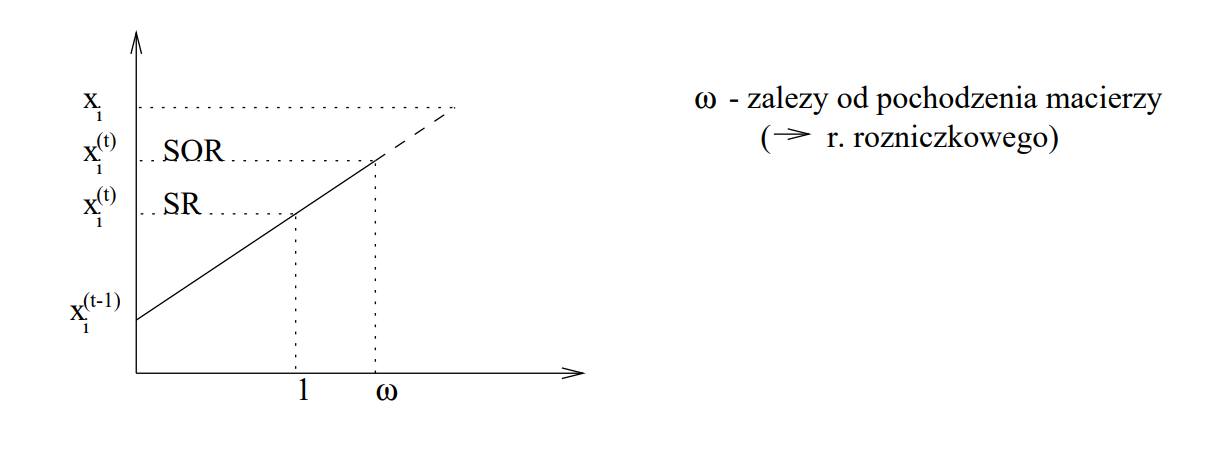
\includegraphics[height=0.6\textheight, width=1\textwidth]{img/12/iteracja2}
\end{frame}

\begin{frame}{}
  \textbf{Twierdzenie}
  \begin{block}{Założenia}
    Dla A - symetrycznej, dodatnio określonej o postacji blokowo - trójprzekątniowej:
    $$
    A=\begin{bmatrix}
    D_1 & U_1 &&&&\\
    L_2 & D_2 & U_2 &&& \\
    &&...&...&&\\
    &&&L_{n-1}&D_{n-1}&U_{n-1}\\
    &&&&L_n&D_n
    \end{bmatrix}
    $$
  \end{block}
\end{frame}

\begin{frame}
  \begin{block}{Teza}
    $$\rho(M_{GS})=\rho^2(M_J)$$
    $$\omega_{opt}=\frac{2}{1+\sqrt{1-\rho(M_{GS})}}$$
    $$\lambda_{SOR}=\omega_{opt}-1$$
  \end{block}
  \begin{exampleblock}{Dla równania modelowego}
    $$\rho=cos^2(\frac{\pi}{N}), \omega_{opt}\approx2(1-\frac{\pi}{N}, \lambda_{SOR}=1-\frac{2\pi}{N})$$
  \end{exampleblock}
\end{frame}




  \section{12.9 Sposoby przeglądania węzłów siatki}

\begin{frame}{}
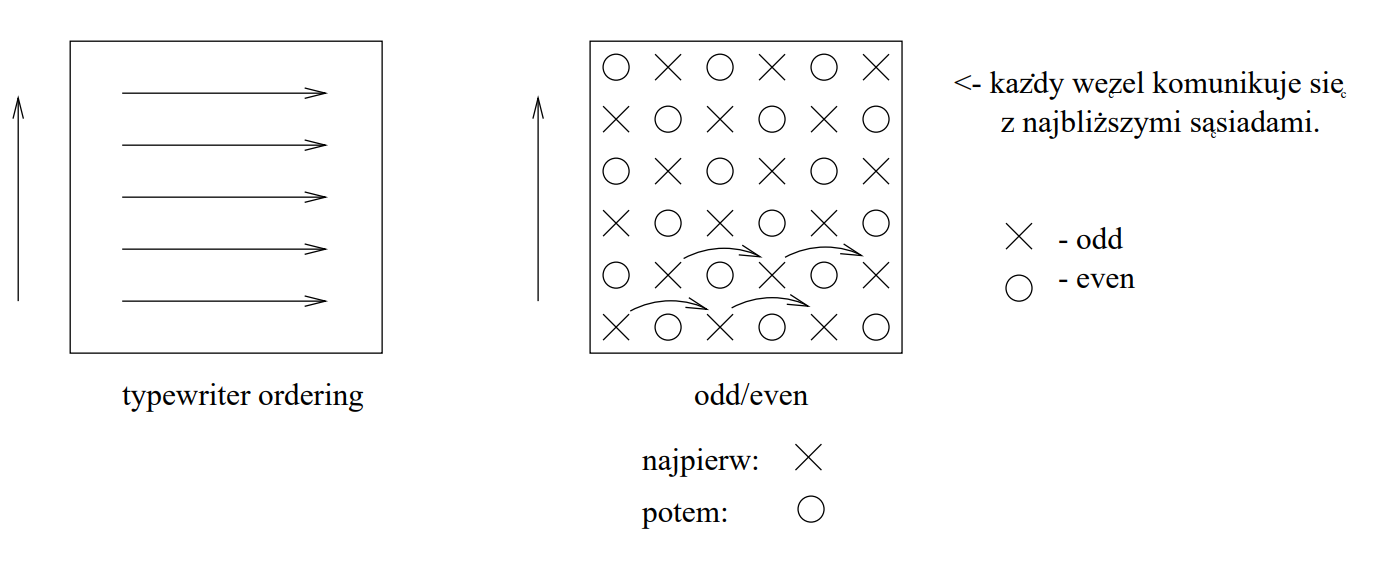
\includegraphics[height=0.6\textheight, width=1\textwidth]{img/12/iteracja3}
\end{frame}


  \section{12.10 Metoda Czybyszewa}

\begin{frame}{Metoda Czybyszewa}
  $B^{-1}=W(A)$ - wielomian macierzowy $M=1-W(A)A$ Znaleźć $W(U)$ taki, by:
  $$minUmax|1-W(U)U|$$
  %prawdopodobnie zły wzór
  Jest to klasyczny problem aproksymacji $\Rightarrow$ wielomiany Czybyszewa
\end{frame}

\begin{frame}
  \begin{block}{Przyspieszenie Czybyszewa metody SOR; odd-even ordering}
    \begin{align*}
    \rho &= \rho(M_J)\\
    \omega^{(0)}&=1\\
    \omega^{\frac{1}{2}}&=\frac{1}{1-\frac{1}{2}\rho^2}\\
    \omega^{(t+\frac{1}{2})}&=\frac{1}{1-\frac{1}{4}\rho^2\omega^{(t)}}\text{, dla t=}\frac{1}{2},1,1\frac{1}{2},...\\
    \omega^{(\infty)} &= \omega_{opt}
    \end{align*}
  \end{block}
\end{frame}

\begin{frame}[fragile]{}
 $\omega=1.0$
\begin{lstlisting}[language=Matlab, mathescape]
DO 2 t = 1, MAXIT$\qquad\qquad\qquad\qquad\qquad (\approx 100,1000)$
    Norm = 0.0
    DO 1 p= 1,n
    DO 1 p= 1,n\\
        IF ( MOD(p+q,2) .EQ. MOD(t,2)) THEN
          Residual = $a_{p,q}\phi_{p,q-1}+b_{p,1}\phi_{p,q+1}+c_{p,q}\phi_{p-1,q}+$
                     $d_{p,q}\phi_{p+1,q}+e_{p,q}\phi_{p,q}-f_{p,q}$
          Norm = Norm + (Residual)$^2$
                 $\phi_{p,q}=\phi_{p_q}-\omega*$Residual$/e_{p,q}$
          ENDIF
    1 CONTINUE
(.) $\omega=1.0/(1.0-0.25\rho^2\omega)$
(.) IF (t .EQ. 1) $\omega=1.0/(1.0-0.5\rho^2)$
    IF (Norm .LT. EPS ||$\overrightarrow{f}$|| solution obtained
2 CONTINUE
\end{lstlisting}
  \hfill\hfill Zadanie: Przećwiczyć na lab.
\end{frame}

\begin{frame}{}
  \begin{block}{Uwagi do algorytmu}
    \begin{itemize}
      \item EPS $\approx 10^{-6}$,
      \item $||f^\rightarrow|| -$ obliczona wcześniej norma prawej strony,
      \item gdy usuniemy instrukcje (*) otrzymamy metodę G-S,
      \item jeżeli dodatkowo zastąpimy $\omega=1$ przez $\omega=\omega_{opt}$-metodę SOR,
      \item (Dla r. Poissona: $a=b=c=d=1, e=-4$)
    \end{itemize}
  \end{block}
\end{frame}



  \section{12.11 Porównywanie jakości wybranych metod iteracyjnych}

\begin{frame}{Porówynwanie jakości wybranych metod iteracyjnych}
  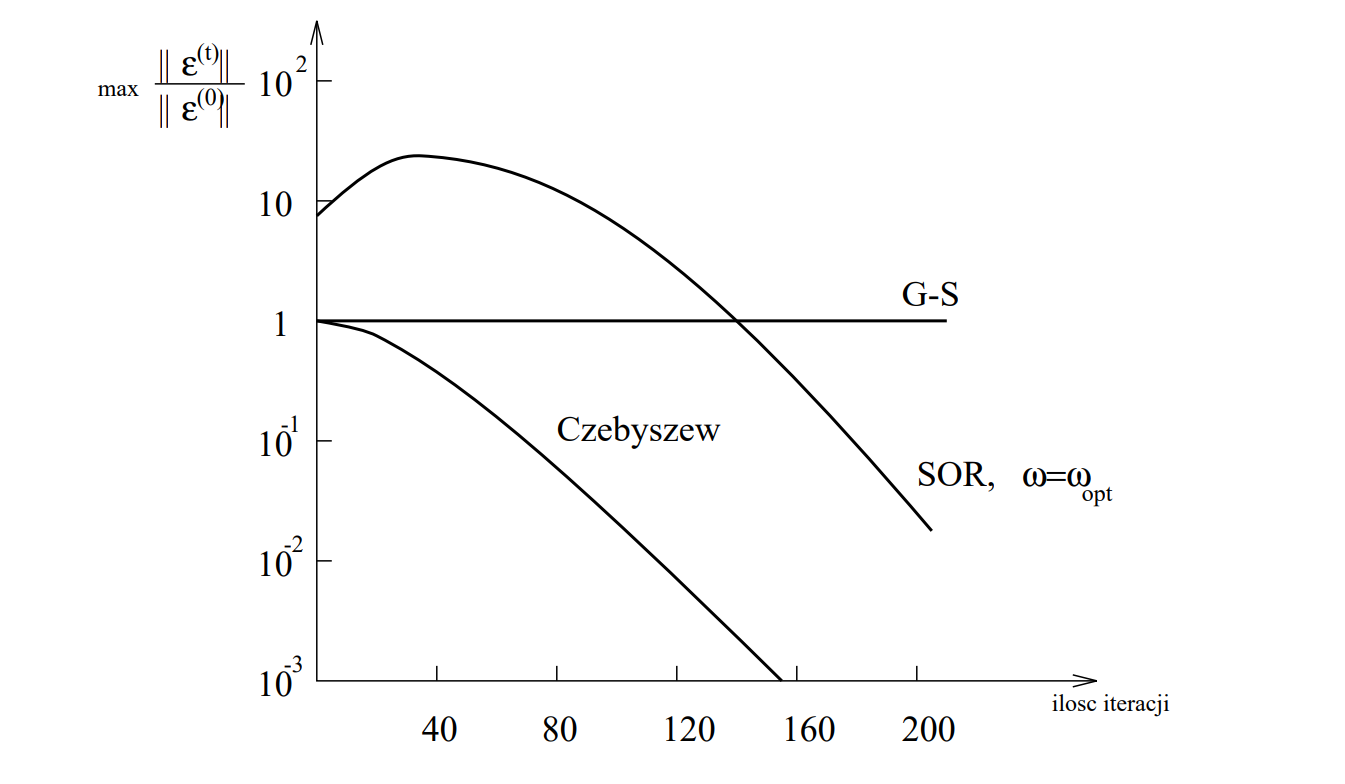
\includegraphics[height=0.5\textheight, width=0.8\textwidth]{img/12/iteracja4}
  $$
  A\leftarrow
  \begin{cases}
    \text{r. Poissona, 2-D}\\
    \text{siatka 128 x 128}
  \end{cases}
  $$
\end{frame}




\end{document}
